% !TEX root = ../main.tex

\chapter{Inspirations}
\label{ch:inspiro}

\startcontents[chapters]
\minicontents

\brule % chktex 1


\section{The Syzygy Surfer}

The research presented here is based on the initial idea of Jim Hendler and Andrew Hugill's ``Syzygy Surfer'' \autocite{Hendler2011, Hendler2013}. They suggest the use of three pataphysical principles, namely clinamen, syzygy and anomaly, to create a new type of Web search engine, reminiscent of the experience of ``surfing the Web''. This is in contrast to current Web search engines which value relevant results over creative ones. \todo{is this my opinion or theirs?} ``Surfing'' used to be a creative interaction between a user and the web of information on the Internet, but the regular use of modern search engines has changed our expectations of this sort of knowledge acquisition. It has drifted away from a learning process by exploring the Web to a straightforward process of information retrieval similar to looking up a word in a dictionary.

\begin{quote}
  ``The ambiguity of experience is the hallmark of creativity, that is captured in the essence of pataphysics. Traversing the representations of this ambiguity using algorithms inspired by the syzygy, clinamen and anomaly of pataphysics, using a panalogical mechanism applied to metadata, should be able to humanize and even poeticize the experience of searching the Web.''\autocite{Hendler2013}
\end{quote}

Their inspirations come from Borges \autocite{Borges2000} (for the underlying poetic sense of unity), Jarry's pataphysical principles \autocite{Jarry1996} and Singh's panalogies (parallel analogies – to introduce ambiguity, since it allows various descriptions of the same object) \autocite{Singh2005}.


\section{Faustroll's Library}

The corpus used resembles the fictional library of ``equivalent books'' from Alfred Jarry's \emph{Exploits and Opinions of Dr.\ Faustroll, $'$Pataphysician} \citeyear[p.10-12]{Jarry1996}\footnote{``In addition, three prints hanging on the walls, a poster by TOULOUSE-LAUTREC, \emph{Jane Avril}; one by BONNARD, advertising the \emph{Revue Blanche}; a portrait of Doctor Faustroll, by AUBREY BEARDSLEY\@; and an old picture, which appeared to us to be valueless, \emph{Saint Cado}, issued by the Oberthuer printing house of Rennes.''\parencite[p.12]{Jarry1996}}.

\begin{enumerate}
\item BAUDELAIRE, a volume of E.A. POE translations.
\item BERGERAC, \emph{Works}, volume II, containing the \emph{Histrory of the States and Empires of the Sun}, and the \emph{History of Birds}.
\item \emph{The Gospel according to} SAINT LUKE, in Greek.
\item BLOY, \emph{The Ungrateful Beggar}.
\item COLERIDGE, \emph{The Rime of the ancient Mariner}.
\item DARIEN, \emph{The Thief}.
\item DESBORDES-VALMORE, \emph{The Oath of the Little Men}.
\item ELSKAMP, \emph{Illuminated Designs}.
\item An odd volume of the \emph{Plays} of FLORIAN\@.
\item An odd volume of \emph{The Thousand and One Nights}, in the GALLAND translation.
\item GRABBE, \emph{Scherz, Satire, Ironie und tiefere Bedeutung}, comedy in three acts.
\item KAHN, \emph{The Tale of Gold and of Silence}.
\item LAUTREAMONT, \emph{The Lays of Maldoror}.
\item MAETERLINCK, \emph{Aglavaine and Selysette}.
\item MALLARME, \emph{Verse and Prose}.
\item MENDES, \emph{Gog}.
\item \emph{The Odyssey}, Teubner's edition.
\item PELADAN, \emph{Babylon}.
\item RABELAIS\@.
\item JEAN DE CHILRA, \emph{The Sexual Hour}.
\item HENRI DE REGNIER, \emph{The Jasper Cane}.
\item RIMBAUD, \emph{The Illuminations}.
\item SCHWOB, \emph{The Childrens' Crusade}.
\item Ubu Roi.
\item VERLAINE, \emph{Wisdom}.
\item VERHAEREN, \emph{The Hallucinated Landscapes}.
\item VERNE, \emph{Voyage to the Center of the Earth}.
\end{enumerate}

\begin{figure}
\centering
\begin{minipage}{.45\linewidth}
  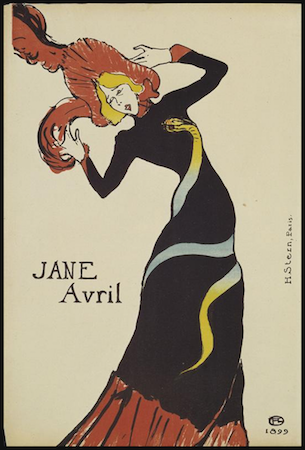
\includegraphics[width=\linewidth]{JaneAvril}
  \caption[Toulouse-Lautrec's ``Jane Avril'']{Toulouse-Lautrec's ``Jane Avril''}
\label{fig:toulouse}
\end{minipage}
\hspace{.05\linewidth}
\begin{minipage}{.45\linewidth}
  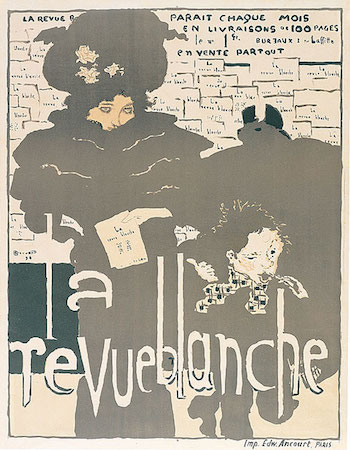
\includegraphics[width=\linewidth]{RevueBlanche}
  \caption[Bonnard's ``Revue Blanche'']{Bonnard's ``Revue Blanche''}
\label{fig:bonnard}
\end{minipage}
\vspace{.05\linewidth}
\begin{minipage}{.45\linewidth}
  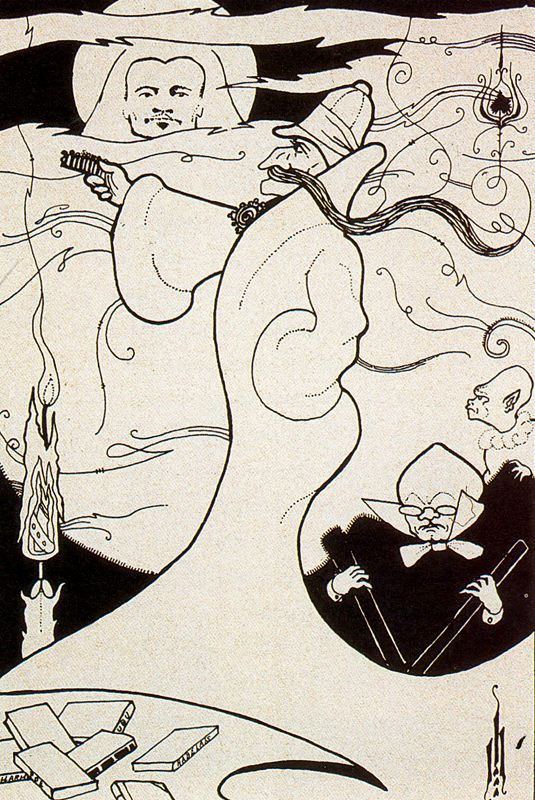
\includegraphics[width=\linewidth]{DocteurFaustroll}
  \caption[Aubrey Beardsley's ``Docteur Faustroll'']{Aubrey Beardsley's ``Docteur Faustroll''}
\label{fig:beardsley}
\end{minipage}
\hspace{.05\linewidth}
\begin{minipage}{.45\linewidth}
  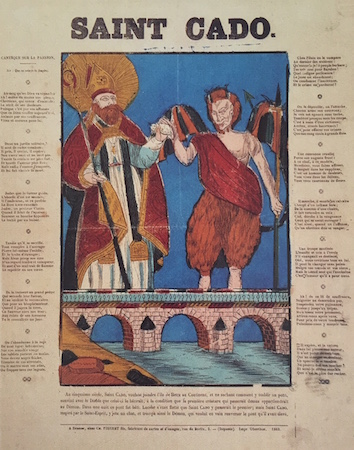
\includegraphics[width=\linewidth]{SaintCado}
  \caption[Oberthuer's ``Saint Cado'']{Oberthuer's ``Saint Cado''}
\label{fig:oberthuer}
\end{minipage}
\end{figure}


\section{100.000.000.000.000 Poems}

Raymond Queneau's `Cent Mille Milliards de Poèmes' is a prime example of Oulipian art. The book is essentially made up of 10 pages containing one sonnet each. Each page however is split into 14 thin strips, one for each line. This means that mathematically there are $10^{14}$ possible poems to be read by combining different lines every time.

\begin{figure}[h!]
\centering
\begin{minipage}{.45\linewidth}
  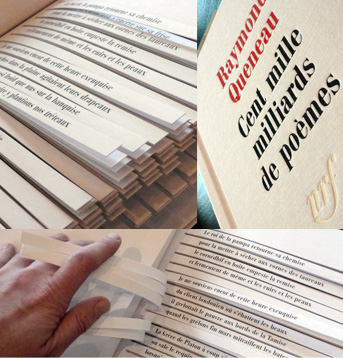
\includegraphics[width=\linewidth]{queneau1}
\end{minipage}
\hspace{.05\linewidth}
\begin{minipage}{.45\linewidth}
  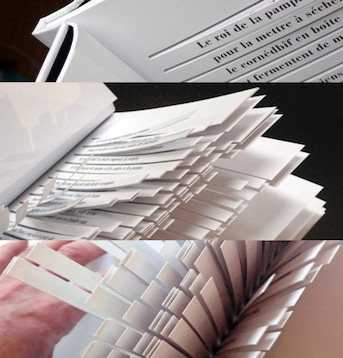
\includegraphics[width=\linewidth]{queneau2}
\end{minipage}
\caption[queneau1+2]{queneau1+2\footnotemark}
\label{fig:queneau12}
\end{figure}
\footnotetext{Images by Martin Pyper \url{http://www.mestudio.info/2010/02/28/one-hundred-thousand-billion-poems/}}
\todo{place footnote text on correct page on final runthrough}


\section{Chinese Encyclopaedia}

Jorge Luis Borges `Chinese Encyclopaedia' in the short story ``The Language of John Wilkins'' \autocite{Borges2000} is a primary inspiration for this project. It lists the following results under the category of `animal'.\todo{check ref}

\begin{quote}
\begin{enumerate}
  \item those that belong to the Emperor,
  \item embalmed ones,
  \item those that are trained,
  \item suckling pigs,
  \item mermaids,
  \item fabulous ones,
  \item stray dogs,
  \item those included in the present classification,
  \item those that tremble as if they were mad,
  \item innumerable ones,
  \item those drawn with a very fine camelhair brush,
  \item others,
  \item those that have just broken a flower vase,
  \item those that from a long way off look like flies.
\end{enumerate}
\end{quote}

Although these are all perfectly valid results, it is clear that they form a more creative, even poetic, view of what an animal might be than the Oxford English Dictionary's prosaic: ``a living organism which feeds on organic matter''.\footnote{``animal, n.''. OED Online. September 2015. Oxford University Press. \url{http://www.oed.com/view/Entry/273779?rskey=qx2uxn&result=1&isAdvanced=false} (accessed December 02, 2015).}


\section{Yossarian Lives}

YossarianLives is a creative search engine which claims to return ``diverse and unexpected results''.\autocite{Yossarian2015}

``These types of results are incredably useful for any one who derives value from new ideas.''\autocite{Yossarian2015}

\begin{quote}
\begin{itemize}
  \item Augmented creativity
  \item Lateral Discovery
  \item Metaphorical Search
  \item Creative Graph
\end{itemize}
\end{quote}\footnote{\url{http://about.yossarianlives.com/index.html}}


\section{The Library of Babel}

The library of babel is \\
created by Jonathan Basile.

\begin{quote}
  The Library of Babel is a place for scholars to do research, for artists and writers to seek inspiration, for anyone with curiosity or a sense of humor to reflect on the weirdness of existence --- in short, it’s just like any other library. If completed, it would contain every possible combination of 1,312,000 characters, including lower case letters, space, comma, and period. Thus, it would contain every book that ever has been written, and every book that ever could be --- including every play, every song, every scientific paper, every legal decision, every constitution, every piece of scripture, and so on. At present it contains all possible pages of 3200 characters, about 104677 books.

  Since I imagine the question will present itself in some visitors’ minds (a certain amount of distrust of the virtual is inevitable) I’ll head off any doubts: any text you find in any location of the library will be in the same place in perpetuity. We do not simply generate and store books as they are requested --- in fact, the storage demands would make that impossible. Every possible permutation of letters is accessible at this very moment in one of the library's books, only awaiting its discovery. We encourage those who find strange concatenations among the variations of letters to write about their discoveries in the forum, so future generations may benefit from their research.\footnote{\url{https://libraryofbabel.info/}}
\end{quote}

\stopcontents[chapters]
